\documentclass[12pt,a4paper]{article}
\usepackage{graphicx}
\usepackage[left=2cm,right=2cm,top=2cm,bottom=2cm]{geometry}
\usepackage[colorlinks = true,
            linkcolor = black,
            urlcolor  = blue,
            citecolor = blue,
            anchorcolor = blue]{hyperref}

\author{Aadityanshu Abhinav ME22B088}
\title{ID2090 Assignment 3}

\date{February 04, 2023}

\begin{document}

\maketitle

\section{ME22B088}

My roll number is {\tt ME22B088} and my GitHub username is {\tt AadityanshuAbhinav}.

\begin{equation}
	[x=16\sin^3(t), y=13\cos(t)-5\cos(2t)-2\cos(3t)-\cos(4t), 0\leq t\leq2\pi]\footnote{\href{https://www.facebook.com/MITnews/videos/valentines-day-2021/335257414441333}{MIT} shared this on Feb 14, 2021 on their Facebook page.}
	\label{eqn:fav}
\end{equation}

Eqn~\ref{eqn:fav} shows a parametric equation, the graph of which is a heart shaped curve shown in fig~\ref{favplot}. Another heart curve may be generated by cardioid of which the polar equation is eqn~\ref{eqn:cardioid}.

\begin{equation}
	r=a(1-\cos{\theta})
	\label{eqn:cardioid}
\end{equation} 

And the graph for eqn~\ref{eqn:cardioid} is as shown in fig~\ref{cardioplot}.

\begin{figure}[h]
	\begin{center}
		\framebox{
			\includegraphics[scale=0.15]{Heart_Parametric.eps}
		}
	\end{center}
	\caption{Screenshot of the heart curve for eqn~\ref{eqn:fav} from video referred in footnote 1}
	\label{favplot}
\end{figure}

\begin{figure}[h]
	\begin{center}
		\framebox{
			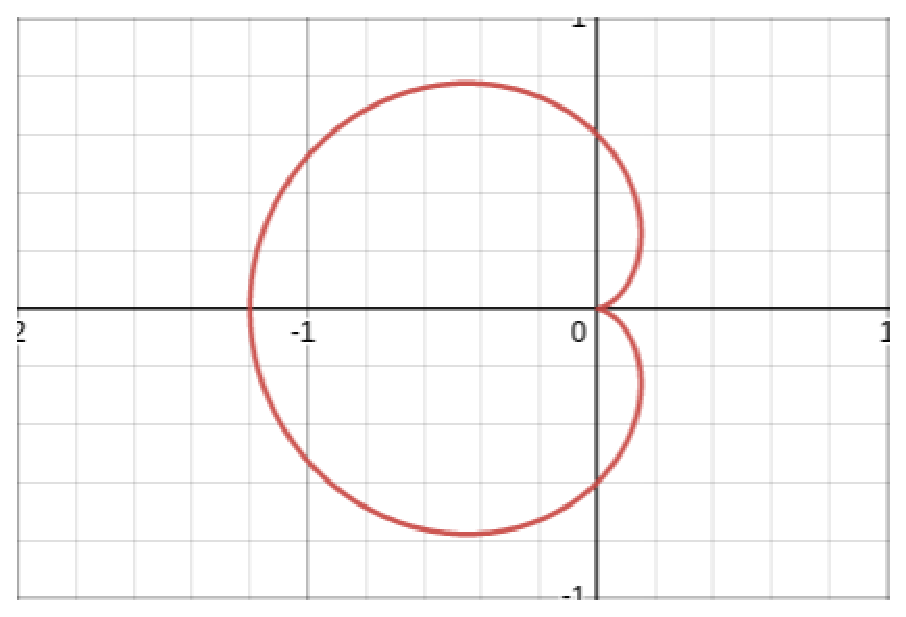
\includegraphics[scale=0.3]{Cardio.eps}
		}
	\end{center}
	\caption{Screenshot of the heart curve for eqn~\ref{eqn:cardioid}}
	\label{cardioplot}
\end{figure}

\end{document}